\documentclass{article}

\usepackage{graphicx,amsmath,arydshln,geometry,float,subfigure,adjustbox,indentfirst} % Required for inserting images

\usepackage[backref, colorlinks=true, linkcolor=black, urlcolor=black, citecolor=black]{hyperref} %目录链接
\usepackage{multirow}

\geometry{a4paper}
\geometry{margin=1in}

\title{\textbf{Final Project Report}}
\author{Wavelix}
\date{}

\begin{document}
\maketitle

\begin{abstract}
    In this project we apply K-Means++, soft K-means, PCA, Nonlinear Autoencoders, MLP SVM, SVM with Gaussian kernel, and AdaBoost on the dataset. The results demonstrate that MLP and AdaBoost achieved the highest accuracy for binary classification tasks, with accuracies exceeding 0.97. Soft K-Means showed greater flexibility and stability compared to K-Means++, particularly with careful selection of the β parameter. Dimensionality reduction techniques, such as PCA and nonlinear autoencoders, effectively simplified the dataset while preserving essential structures, improving clustering performance on reduced dimensions. SVM with Gaussian kernels excelled in handling complex decision boundaries but showed sensitivity to hyperparameter tuning.

    The study highlights the importance of method selection based on dataset characteristics and task requirements, emphasizing that combining complementary approaches can enhance performance and provide deeper insights. Balancing accuracy, computational efficiency, and model complexity is essential for real-world machine learning applications.
\end{abstract}

\tableofcontents % 目录

\section{Introduction}
The project aims to analyze and classify the wheat seed dataset using K-Means++, soft K-means, PCA, Nonlinear Autoencoders, MLP, SVM, SVM with Gaussian kernel, and AdaBoost, and will compare the performance of these methods on both multi-class and binary classification tasks.

\section{Methodology and Solution}
\subsection{K-Means++ Algorithm}
This section aims to apply the K-Means$++$ algorithm to the dataset with K=3 to perform clustering.

The first step is to initialize the center:
\begin{enumerate}
    \item Randomly select the first data point as the initial center using random seeds.
    \item For each remaining data point $x^{(n)}$, compute the squared distance $D(x^{(n)})$ to its nearest centroid.
    \item Construct a probability distribution for selecting the next centroid:
    $$
    P(x^{(n)})=\frac{D(x^{(n)})^2}{\sum_{j}D(x^{(j)})^2}
    $$
    Points farther from existing centroids have a higher probability of being selected. Use the probability to select the next centroid based on the distribution.
    \item Repeat the process until $k$ centroids are chosen.
\end{enumerate} 
Once the initial centroids are determined, assign each data point to the cluster of its nearest centroid. For each point $x^{(n)}$, compute the Euclidean distance to all centroids, and assign the point to the cluster. After assigning samples to clusters, update the centroids based on the current cluster memberships. The new centroid is calculated as the mean of all points in the cluster.

To evaluate clustering performance, compare the predicted clusters with the true labels using accuracy metrics:
$$
\text{Accuracy}=\frac{\text{number of correctly classified samples}}{\text{total number of samples}}
$$

Since different random seeds can influence the results, we choose to repeat the algorithm with various random seeds and calculate the mean accuracy.

\subsection{Soft K-Means Algorithm}
This section aims to apply the Soft K-Means algorithm to the dataset with K=3 to perform clustering.

Firstly, randomly initialize $k$ centroids. Then, calculate responsibility for each point respect to each cluster:
$$
r_k^{(n)}=\frac{\exp [-\beta d(m_k,x^{(n)})]}{\sum_{j}\exp [-\beta d(m_j,x^{(n)})]}
$$
The centroid are updated by computing a weighted mean of the data points:
$$
m_k=\frac{\sum_n r_k^{(n)}x^{(n)}}{\sum_n r_k^{(n)}}
$$
Also, calculate the mean accuracy to evaluate clustering performance.

\subsection{PCA Implementation}
This section aims to use PCA to reduce the dimensionality of the dataset and visualize the principal components with dimension being 2 and 3, respectively.

Firstly, subtract the mean of each features from the data, which ensure the data is centered around the origin. Then, compute the covariance matrix:
$$
C=\frac{1}{n}X^TX
$$
Compute the eigenvalues and eigenvectors of the covariance matrix. Then, Select the top k eigenvectors corresponding to the largest eigenvalues to construct the transformation matrix:$W=[v_1\quad v_2\quad \cdots\quad v_k]$. After that, project the data by $X_{\text{reduced}}=X\cdot W$. The reduced data can be transformed back to the original space to approximate the original data:
$$
X_{\text{reconstructed}}=X_{\text{reduced}}\cdot W^T+\text{mean}
$$
The reconstruction error is calculated by:
$$
\text{reconstruction error}=\frac{1}{n}\sum_{i=1}^{n}|| X_{\text{original}}-X_{\text{reconstructed}} ||^2
$$

\subsection{Nonlinear Autoencoder Implementation}
This section aims to use nonlinear autoencoder to reduce the dimensionality of the dataset and visualize the principal components with dimension being 2 and 3, respectively.

We choose the leaky $\mathbf{ReLU}$ (with $\alpha$=0.01) as the activation function. The reduced dimension is determined by the size of the last hidden layer.

Since the structure and updating process of autoencoder is very similar to that of MLP, here we have no more explanation.

The reconstruction error is also calculated after the training.

\subsection{Clustering with Reduced dimensions}
This section aims to apply K-Means$++$ and Soft K-Means on the reduced dimensions obtained from PCA and Nonlinear autoencoder, and compare the result with the ones obtained by original data. The algorithms are in $\mathbf{KMeansPPReducedDim.py}$ and $\mathbf{SoftKMeansReducedDim.py}$, which just need to import the classes and functions in previous python files.

\subsection{MLP for Multi-Class Classification}
This Section aims to Apply a MLP to solve the multi-class classification problem, and compare the its performance with the clustering results in previous section.

Split the data to training set and test set, with the ratio of 7:3. BGD update is applied during the training process. We choose $\mathbf{ReLU}$ as the activation function for the hidden layers while $\mathbf{Softmax}$ for the output layer.

In forward pass, for each hidden layer:
$$
z=a_{i-1}W+b \qquad a_i=\mathbf{ReLU}(z)
$$
for output layer:
$$
z=a_{i-1}W+b \qquad a_i=\mathbf{Softmax}(z)
$$

The cross-entropy loss is applied to measure the error:
$$
\mathcal{L}=-\frac{1}{m}\sum_{m}\sum_{K}y_{i,k}\log(p_{i,k})
$$

In backward pass, output layer:
$$
\delta^L=a^L-y
$$
$$
\frac{\partial \mathcal{L}}{\partial W^L} = \frac{1}{m}a^{L-1}\delta^L\quad \frac{\partial \mathcal{L}}{\partial b^L}=\frac{1}{m}\sum \delta^L
$$
hidden layer:
$$
\delta^l=(\delta^{l+1}W^{l+1})\cdot f'(z^l)
$$
$$
\frac{\partial \mathcal{L}}{\partial W^l}=\frac{1}{m}a^{l-1} \delta^l \quad \frac{\partial \mathcal{L}}{\partial b^l}=\frac{1}{m}\sum \delta^l
$$

In prediction stage, choose the class with the highest probability. Accuracy is calculated to estimate the performance.

The algorithm also allows binary classification mode.

\subsection{SVM and SVM with Gaussian Kernel}
This section aims to develop algorithm for SVM and SVM with Gaussian kernel using python and numpy.

Here I use the code provided by the professor, which includes the algorithm for SVM and SMO. In $\mathbf{SVM/classify.py}$, both linear SVM and SVM with Gaussian kernel are implemented. Since the original dimension of the dataset is 7, which can not be visualized, I developed the SVM with reduced dimensioned obtained from PCA in $\mathbf{SVM/visualclassify.py}$.

\subsection{AdaBoost Algorithm}
This section aims to develop the AdaBoost algorithm to solve the binary classification problem.

Firstly, change the label of the target to $+1$ and $-1$, then initialize the weights $w=\frac{1}{N}$. Define cost function:
$$
J_m=\sum_{n=1}^{N}w_n^m [y_m(x^n)\ne t^{(n)}]
$$
Weighted error on a class:
$$
\epsilon_m=\frac{J_m}{\sum_{n} w_n^m}
$$
Quality of the classifier:
$$
\alpha=\ln (\frac{1-\epsilon_m}{\epsilon_m})
$$
Update the weights by:
$$
w_n^{m+1}=w_n^m \exp (-\frac{1}{2} t^{(n)} \alpha_m y_m(x^{(n)}))
$$
The prediction is calculated by:
$$
y(x)=\text{sign}\left( \sum_{m=1}^{M} \alpha_m y_m(x) \right)
$$
Accuracy is used to evaluate the performance of the model.

\section{Results and Analysis}
\subsection{Results}
Table~\ref{Table 1} shows the accuracy of K-Means$++$ and Soft K-Means on both original dataset and reduced data, with 100 different random seeds tested on each case.
\begin{table}[H]
    \centering
    \begin{tabular}{|c|cc|cc|cc|cc|cc|}\hline
    \multirow{2}{*}{}       &\multicolumn{2}{l|}{Original Data}&\multicolumn{2}{l|}{PCA 2D}& \multicolumn{2}{l|}{PCA 3D}    & \multicolumn{2}{l|}{AE 2D}    & \multicolumn{2}{l|}{AE 3D}    \\ \cline{2-11} 
                            &\multicolumn{1}{l|}{mean}   &var  &\multicolumn{1}{l|}{mean}  &var   & \multicolumn{1}{l|}{mean}  &var  &\multicolumn{1}{l|}{mean}  &var &\multicolumn{1}{l|}{mean}  &var \\ \hline
    K-Means$++$             &\multicolumn{1}{l|}{0.8532} &0.06 &\multicolumn{1}{l|}{0.9126}&0.28  & \multicolumn{1}{l|}{0.9106}&1.49 &\multicolumn{1}{l|}{0.9116}&0.06&\multicolumn{1}{l|}{0.8992}&0.05\\ \hline
    Soft K-Means $\beta=0.8$&\multicolumn{1}{l|}{0.9048} &0    &\multicolumn{1}{l|}{0.8858}&0     & \multicolumn{1}{l|}{0.8810}&0    &\multicolumn{1}{l|}{0.6667}&0   &\multicolumn{1}{l|}{0.6652}&0.31\\ \hline
    Soft K-Means $\beta=1$  &\multicolumn{1}{l|}{0.8952} &0    &\multicolumn{1}{l|}{0.9000}&0     & \multicolumn{1}{l|}{0.9048}&0    &\multicolumn{1}{l|}{0.8000}&0   &\multicolumn{1}{l|}{0.6622}&0   \\ \hline    
    Soft K-Means $\beta=2$  &\multicolumn{1}{l|}{0.8952} &0    &\multicolumn{1}{l|}{0.9238}&0     & \multicolumn{1}{l|}{0.9238}&0    &\multicolumn{1}{l|}{0.8619}&0   &\multicolumn{1}{l|}{0.9095}&0   \\ \hline
    \end{tabular}
    \caption{Results of K-Means$++$ and Soft K-Means}
    \label{Table 1}
\end{table}

Figure~\ref{Figure 1} shows the visualization of PCA. The reconstruction error for 2D PCA is 0.110175, while for 3D PCA is 0.013318.

\begin{figure}[H]
    \centering
    \subfigure[PCA 2D]{    
    \adjustbox{valign=c}{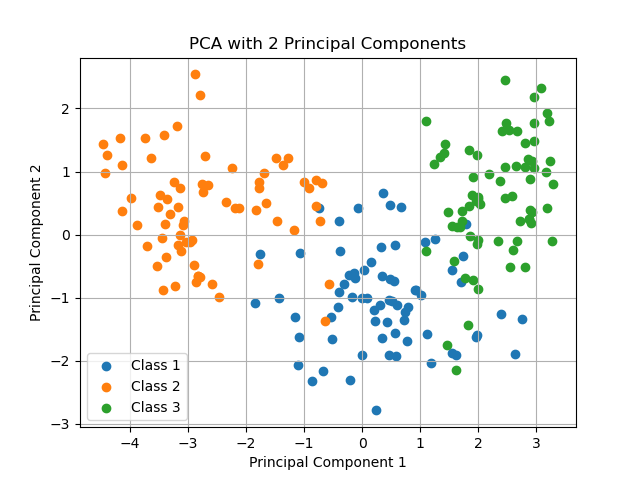
\includegraphics[width=0.45\textwidth]{PCA2D.png}}
    }
    \subfigure[PCA 3D]{
    \adjustbox{valign=c}{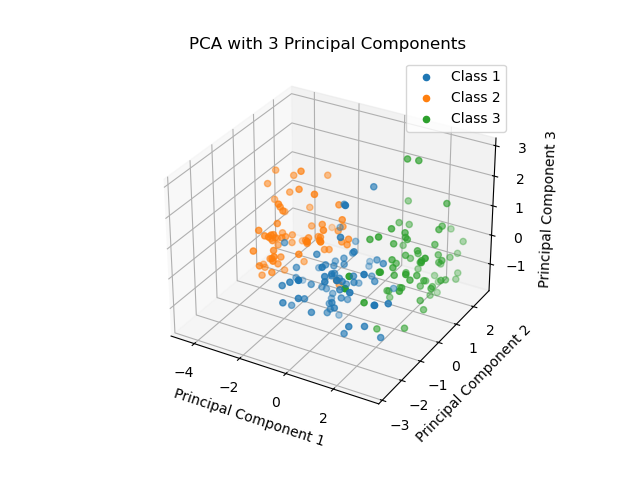
\includegraphics[width=0.45\textwidth]{PCA3D.png}}
    }
    \caption{Visualization of PCA}
    \label{Figure 1}
\end{figure}

Figure~\ref{Figure 2} shows the visualization of nonlinear autoencoder. The reconstruction error for 2D AE is 0.110175, while for 3D AE is 0.013318, the same as PCA.

\begin{figure}[H]
    \centering
    \subfigure[Autoencoder 2D]{    
    \adjustbox{valign=c}{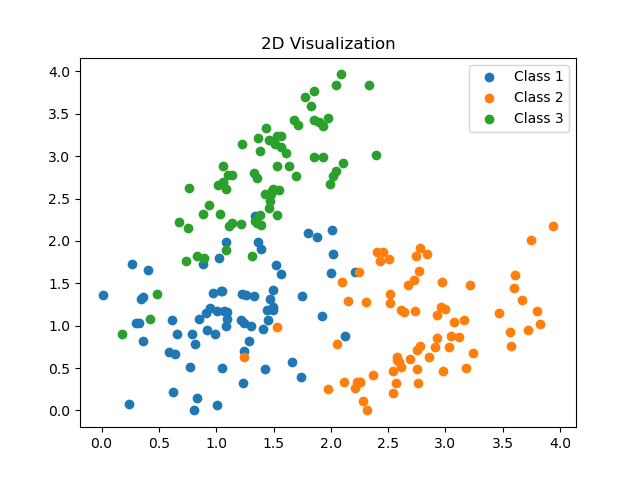
\includegraphics[width=0.45\textwidth]{AE2D.png}}
    }
    \subfigure[Autoencoder 3D]{
    \adjustbox{valign=c}{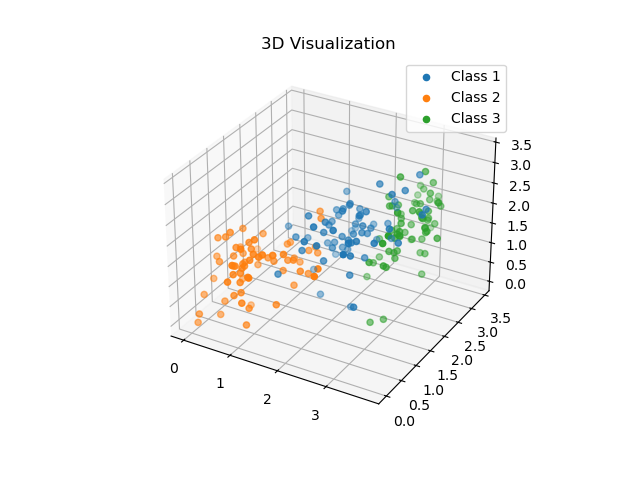
\includegraphics[width=0.45\textwidth]{AE3D.png}}
    }
    \caption{Visualization of Nonlinear Autoencoder}
    \label{Figure 2}
\end{figure}

Figure~\ref{Figure 3} shows the loss curve of MLP for multi-class classification. The final accuracy is 0.9524, with learning rate of 0.1.

\begin{figure}[H]
    \centering
    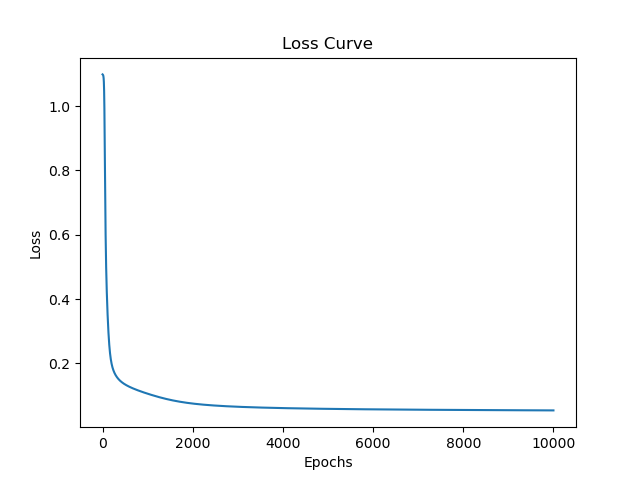
\includegraphics[width=0.5\textwidth]{mcmlp.png}
    \caption{MLP Loss Curve for Multi-Class Classification}
    \label{Figure 3}
\end{figure}

Table~\ref{Table 2} and Table~\ref{Table 3} shows the accuracy of linear SVM and SVM with Gaussian kernel, respectively.

\begin{table}[H]
    \centering
    \begin{tabular}{|c|c|c|c|}\hline
        C&0.1&1&10\\ \hline
        Accuracy&0.9286&0.9500&0.9571\\ \hline    
    \end{tabular}
    \caption{Linear SVM}
    \label{Table 2}
\end{table}

\begin{table}[H]
    \centering
    \begin{tabular}{|c|c|c|c|c|}\hline
        C&0.1&1&10&10\\ \hline
        gamma&scale&scale&scale&auto\\ \hline 
        Accuracy&0.9143&0.9286&0.9357&0.9571\\ \hline   
    \end{tabular}
    \caption{SVM with Gaussian Kernel}
    \label{Table 3}    
\end{table}

Figure~\ref{Figure 3} shows the loss curve of MLP for multi-class classification. The final accuracy is 0.9762, with learning rate of 0.05.

\begin{figure}[H]
    \centering
    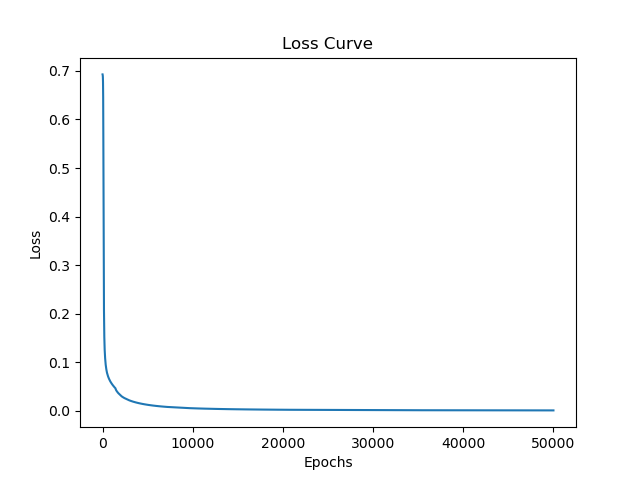
\includegraphics[width=0.5\textwidth]{BMLP.png}
    \caption{MLP Loss Curve for Binary Classification}
    \label{Figure 4}
\end{figure}

For AdaBoost algorithm, we averaged the results generated from different data splitting, and the accuracy can get 0.9967 with the variance less than 0.0002.

\subsection{Analysis}
From Table~\ref{Table 1}, we can compare the performance between K-Means$++$ and Soft K-Means on both original dataset and reduced data. We can draw the following conclusions:
\begin{enumerate}
    \item From the variance of accuracy, we know the Soft K-Means is less sensitive to the initial condition, compared to K-Means++.
    \item The magnitude of $\beta$ can strongly affect the accuracy of Soft K-Means. Smaller $\beta$ is suitable for dataset with ambiguous boundary, while the larger one is suitable for that with clear boundary.
    \item When the data is reduced, K-Means$++$ can have better performance. Different $\beta$ need to be chosen to ensure good performance of Soft K-Means when dimension changes.
\end{enumerate}

For multi-class classification problem, MLP can easily get the highest accuracy over K-Means++ and Soft K-Means. Soft K-Means is more flexible than K-Means++, while $\beta$ can make the clustering process complex. A proper $\beta$ can make Soft K-Means performs better than K-Means++.

$C$ and $Gamma$ can influence the performance of SVM. Larger $C$ tends to make the SVM model strictly fit the data, while may cause overfitting. For SVM with Gaussian kernel, 
when \textit{scale} is applied, $\gamma =\frac{1}{\text{n features}}$, $Gamma$ is only determined by the number of features, while \textit{auto} will consider the variance of the input data.

For binary classification problem, MLP and AdaBoost perform the best, with accuracy larger than 0.97. It's hard to compare the performance of Linear SVM and SVM with Gaussian kernel, since different hyperparameters can lead to different result. Since they have similar results, linear SVM may become a better choice for less hyperparameters.
\paragraph{Advantages and Disadvantages:}
\begin{enumerate}
    \item K-Means$++$ is easy to implement, fast to converge compared to Soft K-Means. However, the initial location of centroid can still affect the overall performance.
    \item Soft K-Means is suitable for fuzzy boundary, and can reduce the likelihood of being stuck in local minima. However, the model is more complex and $\beta$ is difficult to select.
    \item PCA is easy and fast to implement. However, it fails to construct non-linear structure.
    \item Non-linear autoencoder captures non-linear relationships, while the training process can be long and it is sensitive to hyperparameters.
    \item MLP is highly flexible and is suitable for various problems. However, it requires time for training, and has many hyperparameters to choose.
    \item Linear SVM has few hyperparameters, strong generalization ability, and avoids overfitting, while it is limited to linearly separable data.
    \item SVM with Gaussian kernel handles non-linear data well, ideal for complex decision boundaries. However, it has many hyperparameters to choose.
    \item AdaBoost can convert weak classifiers to strong one, and it is highly flexible. However, it is sensitive to noise and outliers, prone to overfitting.
\end{enumerate}


\section{Conclusion}
This project conducted an analysis of the wheat seed dataset using a variety of machine learning techniques, including clustering, dimensionality reduction, and classification methods. Each approach provided unique insights and showed strengths and limitations in addressing the challenges posed by the dataset.

MLP and AdaBoost emerged as the most effective methods for binary classification tasks, achieving high accuracy with proper hyperparameter tuning. Among clustering techniques, Soft K-Means shows greater flexibility and stability compared to K-Means++, particularly with the careful selection of the $\beta$ parameter. Dimensionality reduction techniques such as PCA and nonlinear autoencoders effectively simplified the dataset, preserving essential structures and improving clustering performance on reduced dimensions.

SVM, especially with the Gaussian kernel, excelled in handling complex decision boundaries, although its performance was sensitive to hyperparameter adjustments. Linear SVM and PCA offered simplicity but were limited in capturing non-linear relationships. In contrast, methods like nonlinear autoencoders and MLP provided the flexibility to model complex patterns.

The study highlights the importance of method selection based on the dataset characteristics and task requirements. Combining complementary approaches, as demonstrated, can enhance performance and provide deeper insights. This work underscores the value of balancing accuracy, computational efficiency, and model complexity when choosing machine learning techniques for real-world applications.
\end{document}